\documentclass[12pt]{article}
\usepackage{ficha}

\begin{document}

\ficha{Ângulos e Retas Paralelas}[Retas, Semirretas, Segmentos e Classificação de Ângulos]

\instrucoes{Resolve os exercícios, apresentando os cálculos e justificações. As figuras são esquemáticas e não estão à escala.}

\secao{Ponto, Reta, Semirreta e Segmento}{Responde a cada questão.}

\begin{center}
\begin{tikzpicture}
  \draw[{Latex}-{Latex}] (-0.5,0) -- (6.5,0);
  \foreach \p/\n in {0/A,2/B,4/C,6/D} \fill (\p,0) circle (2pt) node[below] {$\n$};
\end{tikzpicture}
\end{center}

\begin{exercicios}
  \item Quantos segmentos de reta ficam definidos pelos pontos $A$, $B$, $C$ e $D$? Indica-os.
  \item Indica duas semirretas com origem em $B$.
  \item As semirretas $\dot{B}A$ e $\dot{B}C$ são semirretas opostas? Justifica.
  \item Qual é a diferença entre uma reta, uma semirreta e um segmento de reta?
  \item Quantas retas passam por um ponto? E por dois pontos distintos?
  \item O que são retas paralelas? E retas perpendiculares?
  \item O que são retas concorrentes? Duas retas perpendiculares são concorrentes?
  \item Indica, na sala de aula, um exemplo de retas paralelas e um de retas perpendiculares.
\end{exercicios}

\secao{Classificação de Ângulos}{Classifica cada ângulo como agudo, reto, obtuso, raso, giro ou nulo.}
\begin{exercicios}
  \item $35^\circ$
  \item $90^\circ$
  \item $127^\circ$
  \item $180^\circ$
  \item $89^\circ$
  \item $360^\circ$
  \item $91^\circ$
  \item $0^\circ$
  \item Às 3 horas, que ângulo fazem os ponteiros de um relógio? E às 4 horas?
  \item Às 6 horas, que tipo de ângulo fazem os ponteiros?
\end{exercicios}

\secao{Ângulos Complementares e Suplementares}{Calcula o ângulo pedido.}
\begin{exercicios}
  \item O complementar de $30^\circ$.
  \item O complementar de $72^\circ$.
  \item O suplementar de $45^\circ$.
  \item O suplementar de $118^\circ$.
  \item O complementar do complementar de $25^\circ$.
  \item Dois ângulos complementares são iguais. Quanto mede cada um?
  \item Um ângulo é o dobro do seu complementar. Quanto mede?
  \item Um ângulo é o quádruplo do seu suplementar. Quanto mede?
  \item Dois ângulos suplementares diferem $40^\circ$. Quanto mede cada um?
  \item Um ângulo agudo pode ter suplementar agudo? Justifica.
\end{exercicios}

\secao{Ângulos Verticalmente Opostos e Adjacentes}{Observa a figura, onde duas retas se intersetam em $O$, e responde.}

\begin{center}
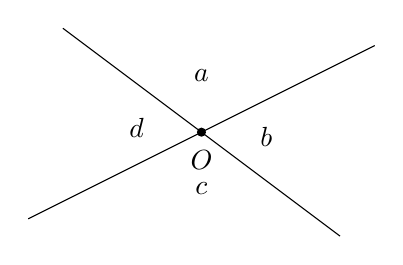
\begin{tikzpicture}[scale=1.1]
  \draw (-2,-1) -- (2,1);
  \draw (-1.6,1.2) -- (1.6,-1.2);
  \fill (0,0) circle (1.5pt) node[below=3pt] {$O$};
  \node at (0,0.65) {$a$};
  \node at (0.75,-0.05) {$b$};
  \node at (0,-0.65) {$c$};
  \node at (-0.75,0.05) {$d$};
\end{tikzpicture}
\end{center}

\begin{exercicios}
  \item Indica dois pares de ângulos verticalmente opostos.
  \item Indica dois pares de ângulos adjacentes e suplementares.
  \item Se $a = 145^\circ$, determina $b$, $c$ e $d$.
  \item Se $b = 38^\circ$, determina $a$, $c$ e $d$.
  \item Se $a = 3x + 10$ e $c = 5x - 30$ (em graus), determina $x$ e a amplitude de todos os ângulos.
  \item Se $a = 2b$, determina a amplitude de cada ângulo.
\end{exercicios}

\secao{Ângulos em Retas Paralelas}{As retas $r$ e $s$ são paralelas e são cortadas pela secante $t$. Observa a figura e responde.}

\begin{center}
\begin{tikzpicture}
  \draw (-2,0) -- (5,0) node[right] {$r$};
  \draw (-2,-2) -- (5,-2) node[right] {$s$};
  \draw (0,1) -- (3,-3) node[below] {$t$};
  \node at (0.95,0.3) {$1$};
  \node at (1.15,-0.3) {$2$};
  \node at (0.4,-0.3) {$3$};
  \node at (0.25,0.3) {$4$};
  \node at (2.45,-1.7) {$5$};
  \node at (2.65,-2.3) {$6$};
  \node at (1.9,-2.3) {$7$};
  \node at (1.75,-1.7) {$8$};
\end{tikzpicture}
\end{center}

\begin{exercicios}
  \item Indica dois pares de ângulos correspondentes.
  \item Indica dois pares de ângulos alternos internos.
  \item Indica dois pares de ângulos alternos externos.
  \item Se o ângulo 1 mede $125^\circ$, determina a amplitude dos restantes sete ângulos.
  \item Se o ângulo 3 mede $120^\circ$, determina os ângulos 5 e 8.
  \item Se o ângulo 2 mede $(2x + 15)^\circ$ e o ângulo 8 mede $(3x - 10)^\circ$, determina $x$.
  \item O ângulo 4 mede $(x + 30)^\circ$ e o ângulo 7 mede $(4x)^\circ$. Justifica que são suplementares e determina $x$.
\end{exercicios}

\secao{Desafios}{Resolve os problemas.}
\begin{exercicios}
  \item Quantos graus roda o ponteiro dos minutos em 20 minutos? E o ponteiro das horas?
  \item Às 2h30, que ângulo fazem os ponteiros do relógio?
  \item Dois ângulos adjacentes formam um ângulo reto e um é o quíntuplo do outro. Quanto mede cada um?
  \item As bissetrizes de dois ângulos adjacentes e suplementares formam que ângulo? Justifica.
  \item Duas retas paralelas são cortadas por uma secante. Um dos oito ângulos formados mede $70^\circ$. Quantos ângulos medem $70^\circ$? E quanto medem os outros?
  \item O suplementar de um ângulo é o triplo do seu complementar. Determina o ângulo.
\end{exercicios}

\end{document}
